\documentclass{article}
\usepackage{graphicx}
\usepackage{amsmath} % define math env \align \endalign
\usepackage{amssymb}% contains the definition of \triangleq,\mathcal
\usepackage{amsfonts}
\usepackage{bm}
\usepackage{mathtools}
\DeclarePairedDelimiter\abs{\lvert}{\rvert}
\DeclarePairedDelimiter\norm{\lVert}{\rVert}
\def\E{\mathbb{E}}
\def\Y{\mathcal{Y}}
\def\T{\mathrm{T}}
\DeclareMathOperator\diag{diag}
\DeclareMathOperator\artanh{artanh}
% decrease the margin as Professor Huang said
% \usepackage[a4paper,margin=2cm]{geometry}
\begin{document}
\begin{figure}[!ht]
\centering
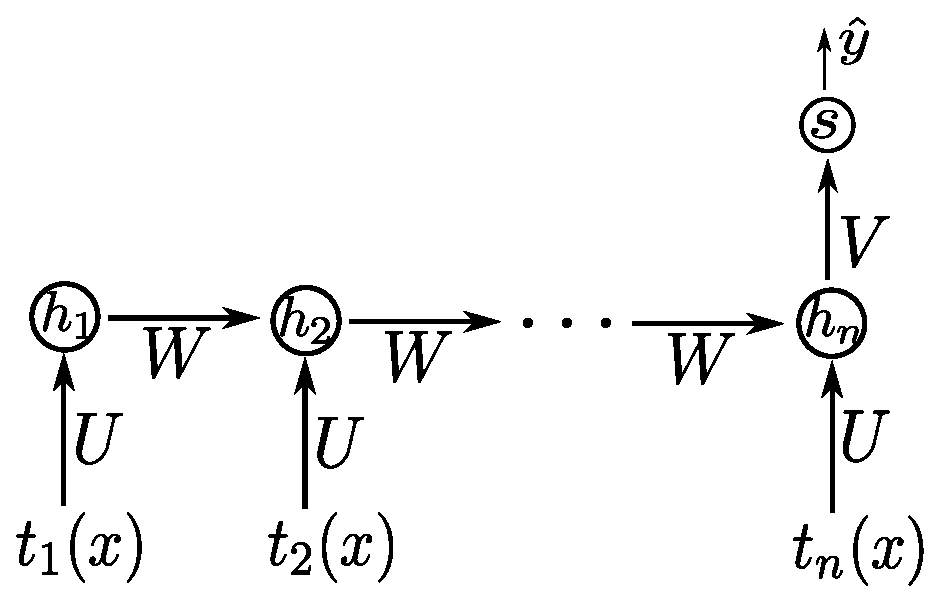
\includegraphics[width=6cm]{rnn.eps}
\end{figure}
% recurrent nerual network
Consider a simple rnn(shown in the figure above), we approximate the distribution $P_{Y|X}$ by the softmax output of rnn: $\widetilde{P}_{Y|X}(k|x) \triangleq \hat{y}_k(x)$. The parameters (mainly matrix $U,W$, $U$ is with dimension $n \times m$ and $W$ is square matrix with dimension $n\times n$) in the different layers of network are shared and are optimized by network training process. We consider special case when $X,Y$ are weakly correlated and the problem is to find the structure of optimal $U$ and $W$ given $V$ and $P_{Y|X}$.

First, we formulate above problem mathmetically. The loss function to minimize has the form (cross entropy loss) 
\begin{equation}\label{eq:cel}
L=-\E_{P_{X,Y}}\log \widetilde{P}_{Y|X}
\end{equation}
(in practial calculation $P_{X,Y}$ is replaced by empirical distribution $\hat{P}_{X,Y}$ which is learned from sample). For rnn network, we have
\begin{subequations}
\begin{align}
\label{eq:h_i} h_i & =  \tanh (W h_{i-1} + U t_i)\\
\label{eq:last_layer} \hat{y}_k & = \frac{\exp(v^T_k h_n+b_k)}{\sum_k \exp(v_k h_n+b_k)},k=1,2,\dots,|\Y|
\end{align}
\end{subequations}
%where $V=[v^\T_1,v^\T_2,\dots,v^\T_{|\Y|}],v_k $ is row vector.
Let $h_i(x,j)$ denotes the $j$\hspace{-0.4pt}-th element of the vector $h_i(x)$, then from \eqref{eq:h_i} we have
\begin{equation}\label{eq:act_item}
h_i(x,j)= \tanh (w_j h_{i-1}(x)+u_j t_i(x,j))
\end{equation}
where $w_j,u_j$ are row vectors respectively.

Suppose $\epsilon$ is  \textbf{small}, and we have the following two assumptions:
\begin{enumerate}
\item $\abs{w_j h_{i-1}(x) - u_j t_i(x,j) }\leq \epsilon$ holds for all $j,i,x$ (former layers) 
\item $|v_k^Th_n-\log P_Y(k)|\leq \epsilon$ holds for all $k$ (last layer)
\end{enumerate}

By Assumption 1 we can expand \eqref{eq:act_item} 
at point zero (use $\tanh' x \vert_{x=0} =1$)as:
$$
h_i(x,j) = w_j h_{i-1}(x) + u_j t_i(x,j) + o(\epsilon)
$$

In matrix notation:

\begin{equation}\label{eq:matrix_step}
h_i(x)=W h_{i-1}(x) + U t_i(x) + o(\epsilon)
\end{equation}

By Assumption 2, the denominator in \eqref{eq:last_layer} can be expanded as ($d(k)\triangleq b_k-\log P_Y(k)$):
\begin{align*}
\sum_{k} \exp(v_k^T h_n + b_k) & = \sum_{k} P_Y(k) \exp(v_k^T h_n + b_k-\log P_Y(k))\\
& = 1 + \E_Y[v(Y)^T] h_n + \E[d(Y)] + {1\over 2}\E_Y[(v(Y)^T h_n+d(Y))^2] + o(\epsilon^2)
\end{align*}
\begin{equation*}
\begin{split}
\log [\sum_{k} \exp(v_k^T h_n + b_k)]  & =    \E_Y[v(Y)^T]h_n  + \E[d(Y)] +\\
& + {1\over 2}\E_Y[(v(Y)^T h_n + d(Y))^2] -{1\over 2}(\E_Y[v(Y)^T]h_n+\E[d(Y)])^2 + o(\epsilon^2)
\end{split}
\end{equation*}
From \eqref{eq:cel}, the loss can be expanded as
\begin{align*}
L & = -\E_{X,Y}[v(Y)^Th_n(X)] -\E[b(Y)]+ \E_X [\log \sum_{k} \exp(v_k^T h_n(X))] \\
& = \E_Y[v(Y)^T]\E_X[h_n(X)]-\E_{X,Y}[v(Y)^Th_n(X)] + H(Y) + \\
& +\frac{1}{2}\E_{X}\E_Y[(v(Y)^T h_n(X)+d(Y))^2]-{1\over 2}\E_X[(\E_Y[v(Y)^T]h_n(X)+E[d(Y)])^2] + o(\epsilon^2) \\
\end{align*}
Equation in \eqref{eq:last_layer} is singular, since adding a constant scalar to $b_k$ or adding a constant vector to $v_k$ does not change the loss function value in \eqref{eq:cel}.
Therefore, we seek the solution $v_k, b_k$, such that $\sum_{k}P_Y(k)b_k=0,\sum_{k}P_Y(k) v_k=\bm{0}$, that is $\E[b(Y)]=0,\E[v(Y)]=\bm{0}$. It can be viewed as minimize \eqref{eq:cel} subject to the two contraints. 

Let $\mu_{h_n}(X)=\E[h_n(X)],\widetilde{h}_n(X)=h_n(X)-\mu_{h_n}(X)$.

Introducing these two constraints, the loss function has the following form:
\begin{align*}
L &= -\E_{X,Y}[v(Y)^T\widetilde{h}_n(X)] + H(Y) +\\
&+\frac{1}{2}\E_X\E_Y[(v(Y)^T\widetilde{h}_n(X))^2] + \E_Y[v(Y)^T\mu_{h_n}(X)+d(Y)]^2 + o(\epsilon^2)
\end{align*}
Let 
\begin{subequations}
\begin{align}
\xi^X(k) & = \sqrt{P_X(k)}\widetilde{h}_n(k)  \\
\xi^Y(k) & = \sqrt{P_Y(k)}v(y)  \\
\Xi^X & = [\xi^X(1),\dots,\xi^X(\abs{\mathcal{X}})]^T \\ % X \times m 
\Xi^Y & = [\xi^Y(1),\dots,\xi^Y(\abs{\mathcal{Y}})]^T    % Y \times m
\end{align}
\end{subequations}
In matrix notation, $\E_X\E_Y[(v(Y)^T\widetilde{h}_n(X))^2]=\norm{\Xi^Y(\Xi^X)^T}^2_F$.

Let $\widetilde{\bm{B}}=\frac{P_{X,Y}(j,i)}{\sqrt{P_X(j)P_Y(i)}}$, which is a $\abs{\mathcal{Y}} \times \abs{\mathcal{X}}$ matrix.

Then $\E_{X,Y}[v(Y)^T\widetilde{h}_n(X)] = \widetilde{\bm{B}}\circ\Xi^Y(\Xi^X)^T $ (Hadamard product).

$\Rightarrow$

\begin{equation}
L = \norm{\widetilde{\bm{B}}-\Xi^Y(\Xi^X)^T}_F^2 + \E_Y[v(Y)^T\mu_{h_n}(X)+d(Y)]^2 + H(Y) -\norm{\widetilde{\bm{B}}}_F^2 + o(\epsilon^2)
\end{equation}

We can make the input $t_i(x)$ have zero mean, then from \eqref{eq:matrix_step} (take the expectation and subtract) we have:
$$
\widetilde{h}_i(x)=W \widetilde{h}_{i-1}(x) + U t_i(x) + o(\epsilon)
$$
We choose $\mu_{h_n}(X)$ to minimize the second term in $L$ and the mean-zero term is our consideration in the following ($\widetilde{B}, \Xi^{Y}$ are both known).

The transpose of $\Xi^{X}$ can be written as
$$
(\Xi^{X})^T = (Ut_n + WUt_{n-1} + \dots + W^{n-1} U t_1) \diag[\sqrt{P_X}]
$$
where $ t_i = [t_i(1), t_i(2), \dots, t_i( \abs{\mathcal{X}} ) ]$ and 
$
\diag [ \sqrt{P_X} ]  = \diag [ P_X(1), P_X(2), \dots, P_X(\abs{\mathcal{X}  })]
$.

To minimize the first term of $L$ about $U,W$ jointly  is difficult. We take an alternative approach. We restrict the square matrix $W$ to such form as $ W = Q \Lambda Q^{-1}, \Lambda =  \diag[\lambda_1,\dots, \lambda_n]$ and $ \widetilde{U} = Q^{-1}U$.
Then
$$
\Xi^Y (\Xi^{X})^T = \Xi^Y (Q\widetilde{U} t_n + Q \Lambda \widetilde{U} t_{n-1} + \dots + Q \Lambda^{n-1} \widetilde{U} t_1 )\diag[\sqrt{P_X}]
$$
Given initial condition $Q_0, \Lambda_0$ and $\widetilde{U}_0$, we use an iterative approach to update from 
$(Q^{(k-1)}, \Lambda^{(k-1)}, \widetilde{U}^{(k-1)})$ to $(Q^{(k)}, \Lambda^{(k)}, \widetilde{U}^{(k)})$.
Since $ \Xi^Y (\Xi^{X})^T$ is linear in $Q$ and $\widetilde{U}$, we can get the closed form expression for either one while fixing the other. Let $ L_1 = \norm{\widetilde{B} - \Xi^Y (\Xi^{X})^T}_F^2 $, the matrix derivative of $L_1$ about $Q$ can be written as:
\begin{equation}\label{eq:Q_iterative}
  (\Xi^Y)^T \widetilde{B} K^T - (\Xi^Y)^T\Xi^Y Q KK^T = 0
\end{equation}
where $ K = (\widetilde{U} t_n + \Lambda \widetilde{U} t_{n-1} + \dots + \Lambda^{n-1} \widetilde{U} t_1)
\diag [ \sqrt{P_X} ] $

Suppose $n<\min\{\abs{\mathcal{X}}, \abs{\mathcal{Y}}\}$, then it is possible for both $ (\Xi^Y)^T\Xi^Y$ and 
$KK^T$ to have inverse matrix. Then 
$$ Q = ((\Xi^Y)^T\Xi^Y)^{-1} (\Xi^Y)^T \widetilde{B} K^T (KK^T)^{-1} $$

To derive the matrix derivative of $L_1$ about $\widetilde{U}$, we flatten $\widetilde{B}, \widetilde{U}$ as one-dimensional vector along each row. That is $\widetilde{U}^T = [\widetilde{u}_1, \dots, \widetilde{u}_n], \widetilde{u}^T = [ \widetilde{u}_1^T, \dots, \widetilde{u}_n^T]$. Similarly we get $\widetilde{b}$ from $\widetilde{B}$. Then
$L_1 = \norm{\widetilde{b} - M \widetilde{u}}_2$ where $ M = \sum_{i=0}^{n-1} \Xi^Y Q \Lambda^i \otimes \diag[\sqrt{P_X}] t_{n-i}^T$. The derivative of $L_1$ about $\widetilde{u}$ is
\begin{equation}\label{eq:U_iterative}
M^T \widetilde{b} = M^T M \widetilde{u}
\end{equation}
Suppose $mn < \abs{\mathcal{X}}\cdot\abs{\mathcal{Y}}$, then it is possible for $M^T M$ to have inverse matrix. Then 
$$ \widetilde{u} = (M^TM)^{-1} M^T \widetilde{b} $$
For the case when either $n<\min\{\abs{\mathcal{X}}, \abs{\mathcal{Y}}\}$ or  $mn < \abs{\mathcal{X}}\cdot\abs{\mathcal{Y}}$ is not satisfied, we can use the regularization method.

Let $\widetilde{L}_1 = L_1 + \lambda \norm{(\Xi_X)^T}_F^2$ and take the derivative...

To update the diagonal matrix $\Lambda $, we update $\lambda_i$ respectively. $L_1$ is a polynomial function about each $\lambda_j$ (the maximal order is $2n-3$).

To update from $\lambda_j^{(k-1)}$ to $\lambda_j^{(k)}$, we use Newton's method:
$$
\lambda_j^{(k)} = \lambda_j^{(k-1)} - \frac{L_1(\lambda_j)}{L_1'(\lambda_j)}
$$
Hence we need the explicit form of $L_1(\lambda_j)$ and $L_1'(\lambda_j)$.

Let $\Lambda_i$ be the diagonal matrix with $\lambda_i$ at $(i, i)$ and zeros at other position. Then
$\Lambda = \sum_{i=1}^n \Lambda_i$. We denote $\widetilde{B}_{\bar{j}}$ (which does not contain $\lambda_j$)as follows:
$$
 \widetilde{B}_{\bar{j}} = \widetilde{B} - \Xi^Y Q \sum_{r=0}^{n-1} \sum_{\substack{i = 1 \\ i \neq j} }^n \Lambda_i^r \widetilde{U} t_{n-r} \diag [\sqrt{P_X}]
$$
Then $L_1(\lambda_j)$ can be written as
$$
L_1(\lambda_j) = \sum_{k, l} = \norm{\widetilde{B}_{\bar{j}} - \Xi^YQ\sum_{r=0}^{n-1} \Lambda_j^r \widetilde{U} t_{n-r} \diag [\sqrt{P_X}] }_F^2
$$

Let $\widehat{Q}_j$ be the j-th column vector of $\Xi^Y Q$ and $\widehat{U}_j(r)$ be the j-th row vector of $\widetilde{U} t_{n-r} \diag [\sqrt{P_X}]$. 
With some computation we have:
$$
L_1'(\lambda_j) = \norm{\widehat{Q}_j}_2^2 \sum_{r'=1}^{2n-2} \sum_{r= 0 }^{r'}  (\widehat{U}_j(r) \cdot \widehat{U}_j(r'-r))
\lambda_j^{r'-1} + \sum_{r = 1}^{n-1} r(\widehat{Q}_j^T \widetilde{B}_{\bar{j}} \widehat{U}_j(r)) \lambda_j^{r-1}
$$

\end{document}

